\documentclass{bioinfo}
\copyrightyear{2015} \pubyear{2015}
\access{Advance Access Publication Date: Day Month Year}
\appnotes{Manuscript Category}

\begin{document}
\firstpage{1}

\subtitle{Data and text mining}

\title[iSEE]{iSEE: Interactive SummarizedExperiment Explorer}
\author[Rue-Albrecht \textit{et~al}.]{Kevin Rue-Albrecht\,$^{\text{\sfb 1,}\dagger}$,
    Federico Marini\,$^{\text{\sfb 2,3,}\dagger}$,
    Charlotte Soneson\,$^{\text{\sfb 4,}\dagger}$,
    and Aaron T. L. Lun\,$^{\text{\sfb 5,}\ast,\dagger}$}
\address{$^{\text{\sf 1}}$Kennedy Institute of Rheumatology, University of Oxford, Oxford OX3 7FY, United Kingdom, \\
$^{\text{\sf 2}}$Center for Thrombosis and Hemostasis (CTH), Mainz \\
$^{\text{\sf 3}}$Institute for Medical Biostatistics, Epidemiology and Informatics, Mainz \\
$^{\text{\sf 4}}$University of Zurich and SIB Swiss Institute of Bioinformatics \\
$^{\text{\sf 5}}$Cancer Research UK Cambridge Institute, University of Cambridge, Cambridge CB2 0RE, United Kingdom \\
$^{^\dagger}$These authors contributed equally.}



\corresp{$^\ast$To whom correspondence should be addressed.}

\history{Received on XXXXX; revised on XXXXX; accepted on XXXXX}

\editor{Associate Editor: XXXXXXX}

\abstract{\textbf{Summary:} Data exploration is critical to the comprehension of large biological datasets generated by high-throughput assays such as sequencing.
However, most existing tools for interactive visualization are limited to specific assays or analyses.
Here, we present the iSEE (Interactive SummarizedExperiment Explorer) software package, which provides a general visual interface for exploring data in a SummarizedExperiment object.
iSEE is directly compatible with many existing R/Bioconductor packages for analyzing high-throughput biological data,
and provides useful features such as simultaneous examination of multiple data aspects, dynamic linking between plots and code tracking for reproducibility.
We demonstrate the utility and flexibility of iSEE by applying it to explore a range of real transcriptomics and proteomics datasets.\\
\textbf{Availability:} iSEE is publicly available as an R package from the open-source Bioconductor project (https://bioconductor.org/packages/iSEE).\\
\textbf{Contact:} \href{aaron.lun@cruk.cam.ac.uk}{aaron.lun@cruk.cam.ac.uk}\\
\textbf{Supplementary information:} Supplementary data are available at \textit{Bioinformatics}
online.}

\maketitle

\section{Introduction}
Interactive data exploration is critical to the analysis and comprehension of the data generated by high-throughput biological assays such as transcriptomics.
Exploration drives the formation of novel data-driven hypotheses prior to a more rigorous statistical analysis, and enables diagnosis of potential problems such as batch effects and low-quality samples.
To this end, visualization of the data in an intuitive and interactive interface is crucial, allowing researchers to examine the data from different perspectives across samples (e.g., experimental replicates, patients, single cells) and features (e.g., genes, transcripts, proteins, genomic regions).

Most existing tools for interactive visualization of biological data are designed for specific assays and analyses, e.g., pRoloc for proteomics \citep{gatto2014mass}, shinyMethyl for methylation \citep{fortin2014shinymethyl}, HTSvis for high-throughput screens \citep{scheeder2017htsvis}.
Opportunities for customization are generally limited, making it difficult to re-use the same visualization software for new technologies or experimental designs where different aspects of the data are of interest.
Moreover, standalone tools such as the Loupe Cell Browser from 10X Genomics \citep{zheng2017massively} do not easily integrate into established analysis pipelines such as those based on the R statistical programming language \citep{rcore2008R}.
This complicates any coordinated use of these tools with a reproducible, transparent, and statistically rigorous analysis.

\begin{figure*}[t]
\includegraphics[width=\textwidth]{pics/Fig1.pdf}
\caption{iSEE uses a customisable multi-panel layout (A) that simultaneously displays one or more panels of various types, where each panel type visualizes a different aspect of the data.
New panels of any type can be added (i), and all panels can be removed, reordered or resized (ii).
Panel types are available visualize sample-based reduced dimensionality embeddings (iii), sample-level metadata (iv), and experimental observations across samples for each feature (v).
For these panel types, each sample is represented as a point, which can be coloured according to sample-level metadata or feature-level observations.
Depending on whether the variables of interest are categorical or numeric, panels will automatically switch between scatter plots, violin plots or ``rectangle plots'' (where each combination of categorical levels is represented by a rectangle with area proportional to the frequency of combination).
Other panel types include row statistics tables (vi), to facilitate searching across features and their metadata; heatmaps (vii), to visualize experimental observations for multiple features; and feature-level metadata plots.
(B) Information can be transmitted between panels according to a user-specified scheme.
Here, the selection of feature $X$ in the row statistics table determines the y-axis of the feature expression plot, and colours the samples in the reduced dimension plot by the expression of $X$.
Selection of points in the reduced dimension plot (dotted blue line) also determines the samples that are shown in the column data (i.e., sample metadata) plot;
further selection of points in the column data plot determines the samples that are shown in the heatmap.
}
\label{fig:iSEE}
\end{figure*}

\section{Description of the iSEE interface}
Here, we present the iSEE software package for interactive data exploration.
iSEE is implemented in R using the shiny framework \citep{chang2017shiny} and exploits data architectures from the open-source Bioconductor project \citep{gentleman2004bioconductor}.
The iSEE interface is initialized with a single function call accepting a SummarizedExperiment object as input \citep{huber2015orchestrating}.
This object stores one or more matrices of experimental observations as ``assays'', where columns and rows represent samples and features, respectively.
Per-feature or per-sample variables are stored in the ``rowData'' and ``colData'', respectively; this includes experimental metadata as well as any analysis results.
All of these data aspects can be directly examined in the multi-panel layout of the iSEE interface (Fig.~\ref{fig:iSEE}A).
The flexibility of the SummarizedExperiment class is the driving factor behind its broad deployment throughout the Bioconductor ecosystem, with uses in RNA sequencing \citep{love2014moderated}, methylation \citep{aryee2014minfi} and Hi-C analysis pipelines \citep{lun2016infrastructure}, amongst others.
By accepting a SummarizedExperiment object, iSEE immediately offers interactive visualization for a variety of data modalities, complementing the state-of-the-art analysis methodologies already available in R/Bioconductor packages.
%In particular, we leverage off the state-of-the-art allowing us to avoid re-implementing them in iSEE (as is commonly done in other standalone visualization tools).

A key feature of iSEE is the ability to dynamically transmit information between panels (Fig.~\ref{fig:iSEE}B).
Users can define arbitrary links between ``transmitting'' and ``receiving'' plots, whereby selection of points on the transmitting plot will highlight the corresponding points in the receiving plot.
This facilitates exploration of the relationships between different aspects of the data -- for example, users can easily determine co-expression patterns of genes in a particular region of a reduced dimensionality embedding, by transmitting information from the reduced dimension plot to one or more feature expression plots.
The linking paradigm extends to multiple plots whereby a plot can transmit to multiple receivers, or a receiving plot can itself transmit to another plot.
This allows users to mimic the arbitrarily complex gating strategies often found in analyses of flow cytometry data \citep{finak2014opencyto}, with the advantage of being extensible to any (meta)data present in a SummarizedExperiment object.
Information can similarly be transferred between tables and plots, e.g., selecting a row determines how points are coloured in receiving plots.

iSEE also offers a host of other customizable features to improve data exploration.
Users can supply their own colour mappings to iSEE, to control how colour scales are chosen for each metadata variable and assay type across all panels in the application.
Row statistics tables can be augmented with dynamic annotation based on the selected row, linking to online resources such as Ensembl or Entrez. % do we need to cite them? at least ENSEMBL has updated citable papers
For large datasets, points can be downsampled in a density-dependent manner to accelerate rendering of the plots, improving the responsiveness of the interface without compromising the fidelity of the visualization.
After analyses are completed, users can deploy iSEE on a server with a bespoke step-by-step ``tour'' of their dataset, guiding the audience through an examination of the salient features in the data.
iSEE also automatically memorizes the exact R code that was used to generate every plot and the existing links,
extending previous work by \cite{marini2016interrepro}.
This allows users to easily reproduce the results of any exploratory analysis, simply by copying the code reported by iSEE into their own analysis scripts.

\section{Conclusion}
iSEE provides a general interactive interface for visual exploration of a diverse range of `-omics datasets.
We provide a number of demonstrations at https://github.com/LTLA/iSEE2018, using iSEE to explore the TCGA RNA-seq collection \citep{piccolo2015TCGA}, the 68,000 PBMC single-cell RNA sequencing dataset from 10X Genomics \citep{zheng2017massively} and a published mass cytometry dataset consisting of over 170,000 cells (CITE?).

\section*{Acknowledgements}
We thank the organizers and participants of the European Bioconductor Meeting 2017, where the idea for this package was first conceived.
We also thank members of the Bioconductor community for their helpful suggestions.
\vspace*{-12pt}

\section*{Funding}
ATLL was supported by core funding from Cancer Research UK (award no. 17197 to Dr.\ John Marioni).
The work of FM is supported by the German Federal Ministry of Education and Research (BMBF 01EO1003).
\vspace*{-12pt}

%\bibliographystyle{natbib}
%\bibliographystyle{achemnat}
\bibliographystyle{plainnat}
%\bibliographystyle{abbrv}
%\bibliographystyle{bioinformatics}
%
%\bibliographystyle{plain}
%
\bibliography{ref}

\end{document}
